\section{Transferability to extended tasks}
The experiments in Section~\ref{sec:umms} established that knowledge transfer between understanding and generation occurs in UMMs with certain architectural properties, and that for counting, this transfer is bi-directional. A natural follow-up question is whether similar patterns hold for other tasks. We investigate this by extending our analysis to two additional domains: OCR, where understanding and generation share character-level visual patterns, and spatial reasoning, where both tasks rely on relative object locations. Throughout this section, we use Lumina-DiMOO~\cite{xin2025lumina} with LoRA-based supervised fine-tuning, as it exhibited the strongest cross-task transfer in the preceding experiments.

\subsection{Text recognition and generation}
We first examine text recognition~(OCR) and text-contained image generation as a pair of complementary tasks. Both tasks operate on character-level visual cues such as strokes, spacing, and glyph structure, requiring the model to capture highly localized and fine-grained visual details. We investigate whether learning such details through one objective transfers to the other.

% \begin{figure*}[t]
%     \centering
%     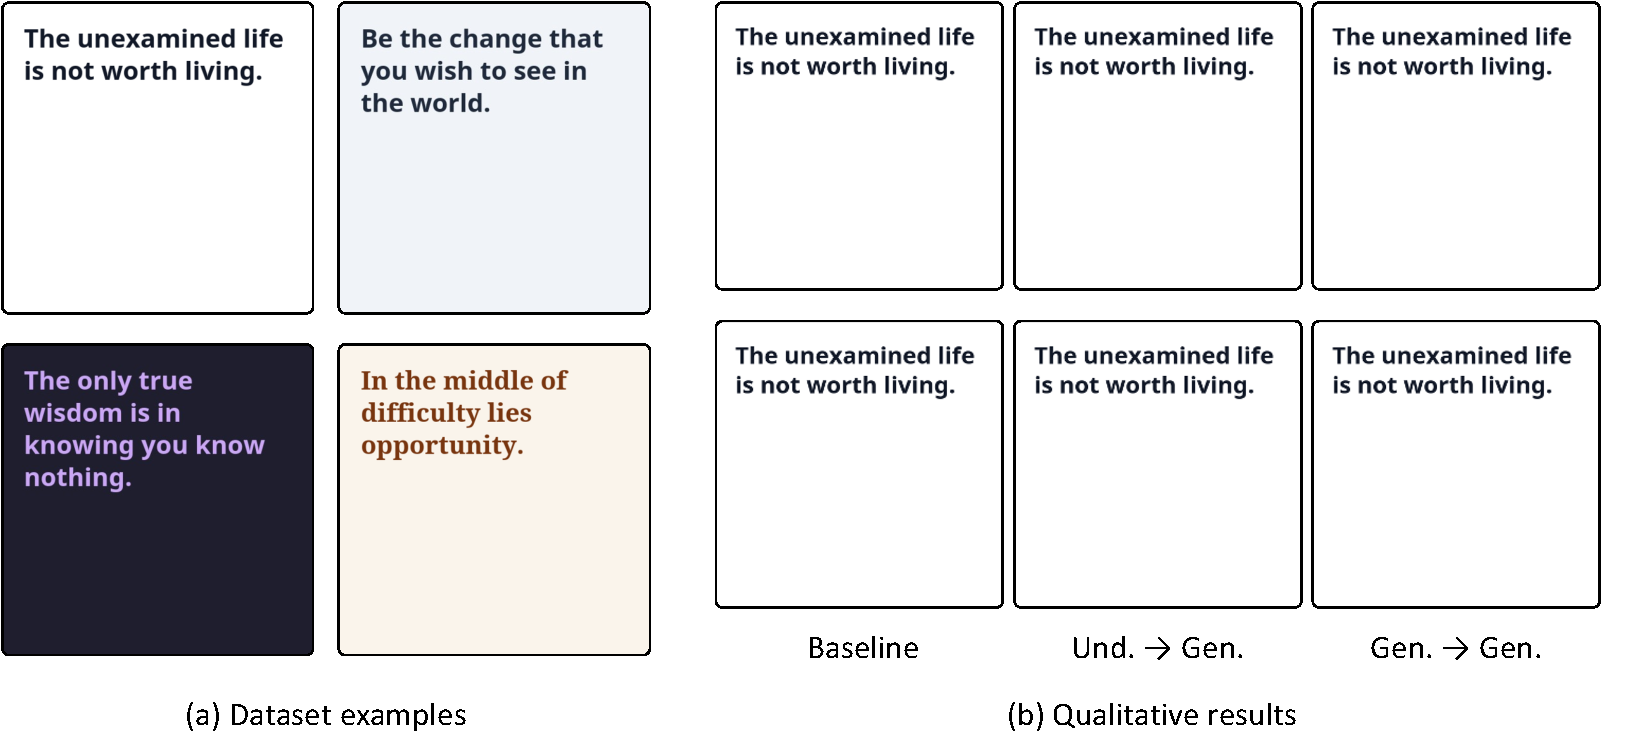
\includegraphics[width=\linewidth]{fig/files/ocr_data_qual.pdf} 
% \caption{(a) Examples from our synthetically rendered Markdown dataset used for both text recognition and text generation training. (b) Qualitative results of text-conditioned image generation under three conditions: Baseline (no fine-tuning), Und.$\rightarrow$
% Gen. (trained only on text recognition), and Gen.$\rightarrow$Gen. (trained and evaluated on text generation).}  
% \label{fig:ocr_data_qual}
% \end{figure*}
\begin{wrapfigure}[15]{r}{0.33\linewidth}
    \centering
    \vspace{-20pt}
    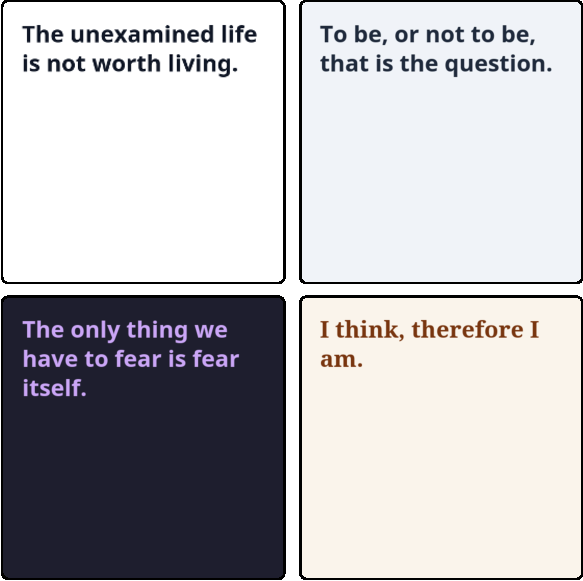
\includegraphics[width=\linewidth]{fig/files/ocr_dataset.pdf}
    \vspace{-5pt}
    \caption{\textbf{Dataset for text recognition and generation.} }
    \label{fig:ocr_dataset}
    \vspace{-40pt}
    \end{wrapfigure}

\subsubsection{Experimental setting.} We construct a dataset of 200K image-text pairs by rendering Markdown documents into images. Existing OCR benchmarks~\cite{} tend to focus on either short sign-level text in natural scenes or dense full-page documents. Neither setting allows meaningful variation in both recognition and generation. Our rendered dataset provides diverse text content at a moderate difficulty level where both tasks can exhibit measurable room for improvement. 
For evaluation, We report five metrics. word error rate (WER) and character error rate (CER) measure exact correctness at the word and character level. Edit Distance captures the minimum number of operations needed to align the prediction with the ground truth. METEOR~\cite{banerjee2005meteor} and F1 assess partial matches by accounting for token overlap and ordering. For understanding, these metrics are computed between the model's output and the ground-truth text. For generation, we first apply an OCR model~\cite{glmocr} to read text from the generated image and then compute the same metrics against the original prompt.
\begin{table*}[!t]
\centering
\begin{tabular*}{\textwidth}{@{\extracolsep{\fill}}cc|cccccc}
\toprule
\multicolumn{2}{c|}{\textbf{Train $\rightarrow$ Test}} 
& \textbf{WER}
& \textbf{CER}
& \textbf{Edit Dist.}
& \textbf{BLEU}
& \textbf{METEOR}
& \textbf{F1}
\\
\midrule

\multirow{2}{*}{Baseline} 
& Und. &  &  &  &  &  &   \\
& Gen. &  &  &  &  &  &   \\
\midrule

\multicolumn{2}{c|}{Und. $\rightarrow$ Und.} &  &  &  &  &  &  \\
\multicolumn{2}{c|}{Und. $\rightarrow$ Gen.} &  &  &  &  &  &  \\
\midrule
\multicolumn{2}{c|}{Gen. $\rightarrow$ Und.} &  &  &  &  &  &  \\
\multicolumn{2}{c|}{Gen. $\rightarrow$ Gen.} &  &  &  &  &  &  \\
\bottomrule
\end{tabular*}
\caption{OCR results of Lumina}
\label{tab:transfer}
\end{table*}

\subsubsection{Generation training improves recognition but not the reverse.} Table~\ref{tab:ocr} summarizes the OCR transfer results. A clear asymmetry emerges between the two transfer directions. Training with the generation objective alone leads to consistent improvement in OCR accuracy across models (\textit{gen}\ $\rightarrow$ \textit{und}). In contrast, training with the understanding objective yields limited gains in text rendering quality (\textit{und}\ $\rightarrow$ \textit{gen}). We attribute this asymmetry to the nature of the two tasks. This contrasts with the counting results in Section~\ref{sec:umms}, where bi-directional transfer was observed.

\subsection{Spatial relation}
\label{sec:spatial_rel}
The previous experiments focus on fine-grained visual details at the character level. We now shift to spatial position, where the model must reason about the coarse layout of objects in a scene. Unlike OCR, spatial reasoning requires understanding semantic relationships between objects rather than local visual patterns. We ask whether learning to recognize spatial arrangements transfers to generating them, and vice versa.

\begin{figure*}[t]
    \centering
    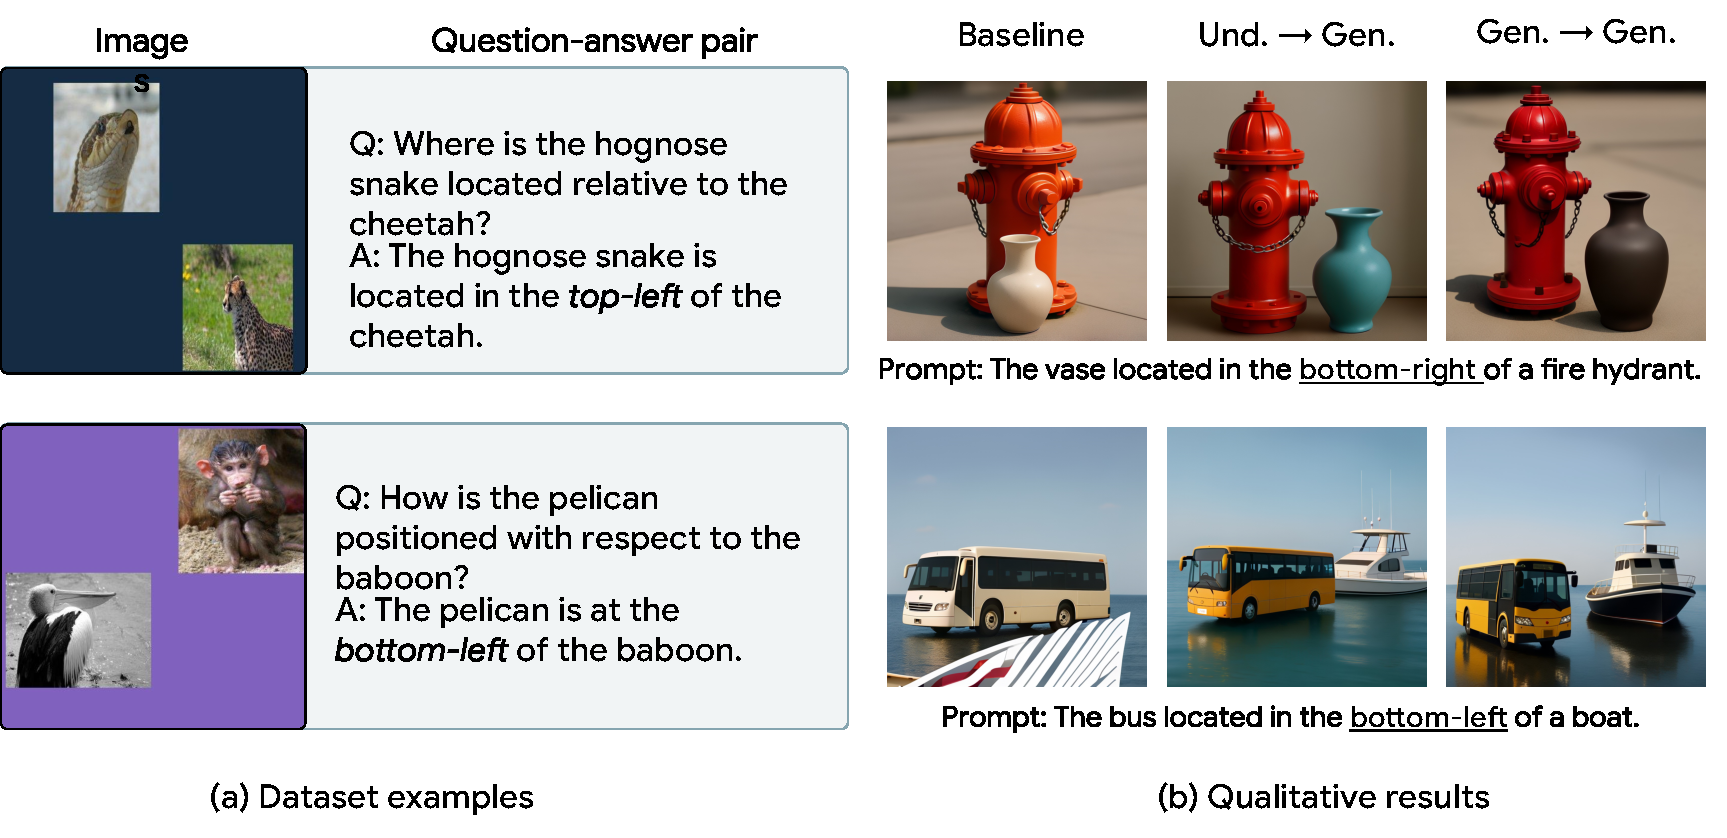
\includegraphics[width=\linewidth]{fig/files/spatial_relation_v2.pdf} 
    \vspace{-5pt}
    \caption{TBD, spatial position}
    \label{fig:spatial_pos}
    \vspace{-5pt}
\end{figure*}


\subsubsection{Experimental setting.} The pre-trained models already handle simple spatial relations such as left, right, top, and bottom reasonably well. We therefore focus on a more challenging setting: diagonal relations between two objects (e.g., top-left, top-right, bottom-right, bottom-left). Since existing spatial reasoning datasets~\cite{} lack the scale and complexity needed for fine-tuning, we construct a synthetic dataset of 200K samples from ImageNet~\cite{}. For each sample, we select two class-image pairs and place them on a canvas according to a randomly sampled diagonal direction. Each sample is paired with a prompt of the form \texttt{"[class A] is located in the [direction] of [class B]"}.
\begin{wraptable}{r}{0.4\textwidth}
    \centering
    \vspace{-20pt}
    \resizebox{0.33\textwidth}{!}{%
        \begin{tabular}{c|c}
            \toprule
            \textbf{Train} 
            & \textbf{Acc.}~$\uparrow$
            \\
            \midrule
            \rowcolor{gray!15}
            \multicolumn{2}{l}{\textit{Understanding}} \\
            Baseline 
            & 0.61 \\
            Und. $\rightarrow$ Und.
            & 0.89 \good{+0.28} \\
            Gen. $\rightarrow$ Und.
            & 0.67 \good{+0.06} \\
            \midrule
            \rowcolor{gray!15}
            \multicolumn{2}{l}{\textit{Generation}} \\
            Baseline
            & 0.67 \\
            Und. $\rightarrow$ Gen.
            & 0.74 \good{+0.07} \\
            Gen. $\rightarrow$ Gen.
            & 0.80 \good{+0.13} \\
            \bottomrule
        \end{tabular}
    }
    \caption{}
    \label{tab:spatial_position_transfer}
    \vspace{-20pt}
\end{wraptable}
For evaluation, understanding is assessed by presenting images in the same format and asking the model to select the correct direction from multiple choices. For generation, we construct prompts in the same format as the training data. Following GenEval~\cite{ghosh2023geneval}, generated images are evaluated by applying a detection model~\cite{} to localize bounding boxes of the two objects. We compute the center points of the detected boxes and verify whether their relative position matches the specified direction.

\subsubsection{Spatial knowledge transfers bi-directionally.} 
Figure~\ref{fig:spatial_pos} summarizes the results. Training with the understanding objective alone improves generation accuracy. Training with the generation objective alone similarly improves understanding. The magnitude of transfer is comparable in both directions. This pattern is consistent with the quantity-aware reasoning results in Section~\ref{sec:umms} and contrasts with the asymmetric transfer observed in text recognition and generation.
